\documentclass[conference]{IEEEtran}
\usepackage{hyperref}
\usepackage{listings}
\usepackage{xcolor}
\usepackage{graphicx}
\usepackage{amsmath}
\usepackage{cite}
\usepackage{url}
\def\UrlBreaks{\do\/\do-\do_\do.}
\graphicspath{{../figures/}}

% Code styling for Solidity
\lstdefinestyle{solidity}{
    language=Java,
    basicstyle=\ttfamily\footnotesize,
    numbers=none,
    frame=single,
    breaklines=true,
    keywordstyle=\color{blue},
    commentstyle=\color{green!60!black},
    stringstyle=\color{red},
    showstringspaces=false,
    xleftmargin=2em,
    framexleftmargin=1.5em
}

\begin{document}

\title{In-Depth Analysis of Alternative Solutions in Solidity Smart Contracts}

\author{
    \IEEEauthorblockN{SHAO Yuning}
    \IEEEauthorblockA{
        Department of Computing\\
        The Hong Kong Polytechnic University\\
        Hong Kong SAR, China\\
        Email: 24045081g@connect.polyu.hk
    }
}

\maketitle

\begin{abstract}
In this paper, we provide an in-depth analysis of similar implementations with different functionalities in smart contracts, based on the Official Developer's Guide for Ethernet. Starting in Chapter 2, we provide a multi-dimensional comparative analysis, followed by a physical storage and logical level security analysis in Chapter 3, and a detailed gas cost comparison in Chapter 4. Finally, we provide recommendations for novice developers.

Keywords: Development, Smart Contract, Security, Gas Optimization
\end{abstract}

\section{Introduction}
Solidity is an object-oriented high-level programming language specifically designed to implement smart contracts on various blockchain platforms (especially the Ethernet blockchain). It was developed by core contributors to the Ethernet network and is statically typed with support for inheritance, libraries, and complex user-defined types\cite{wikiSolidity}. The language is influenced by C++, Python and JavaScript, and is designed specifically for the Ethernet Virtual Machine (EVM).
As Ether continues to dominate the smart contract platform space, more and more developers are adopting Solidity as their primary language for smart contract development. However, for newcomers to blockchain development, Solidity presents unique challenges, especially when it comes to distinguishing between similar implementations that serve the same purpose. This article provides a detailed analysis of these alternatives to help developers write smart contracts using the right approach.

\vspace{3em}
\section{Comparative Analysis}

\subsection{Require vs. Assert vs. Revert}
\subsubsection{Background and Implementation}
A lot of dapps use ownable, we need to do owner validation before calling the function, if it does not meet the rollback occurs. Starting with version 0.4.10 \cite{solidity080}, the traditional throw keyword was replaced by three specialized functions, require(), assert() and revert(), which marked a significant shift in error handling. While all three mechanisms enable transaction rollback, each has different responsibilities.

\begin{lstlisting}[style=solidity]
if(msg.sender != owner) { revert("Not owner!"); } // We can set the return value
assert(msg.sender == owner);
require(msg.sender == owner, "Not owner!"); // We can set the return value
\end{lstlisting}

While these implementations yield identical results, their intended use cases and implications differ significantly in contract design and gas optimization.

\subsubsection{Comparative Analysis}
require() is mainly used to handle input validation and business logic checking, and its concise syntax and gas return mechanism make it ideal for everyday validation; assert() focuses on invariant checking, and plays an important role especially when dealing with overflow/underflow detection and stateful validation; and revert() provides a more flexible approach to error handling, and is especially suited to handling complex conditional branching and custom error scenarios.

In Solidity 0.8.0, the implementation of assert() underwent a significant change from using INVALID to REVERT, an improvement that significantly improves the efficiency of gas while maintaining the ability to roll back state, i.e., it does not consume all the gas, but instead returns it, as with require and reverse. This evolution reflects Solidity's continued efforts to strike a balance between security and efficiency. In practice, developers need to choose the right error handling mechanism according to specific scenarios: for regular input validation, require() is the best choice; for critical invariant checking, assert() should be used; and when complex logic or custom error messages need to be handled, revert() provides the necessary flexibility. This structured error handling strategy not only improves the robustness and gas efficiency of the contract, but also effectively guards against potential security vulnerabilities through a reasonable error handling mechanism.


\vspace{1em}
\subsection{Modifier vs. Direct Function Validation}
\subsubsection{Background and Implementation}

As mentioned above, there are a number of ways in which we can add conditional restrictions \cite{solidityModifiers}. Although these two approaches serve the same purpose, they show significant differences in terms of code reusability, readability and gas consumption.

\begin{lstlisting}[style=solidity]
// Using modifier
modifier onlyOwner() {
    require(msg.sender == owner, "Not owner!!");
    _;
}

function transferOwnership(address newOwner) public onlyOwner {
    owner = newOwner;
}

// Using direct function validation
function transferOwnership(address newOwner) public {
    require(msg.sender == owner, "Not owner!!");
    owner = newOwner;
}
\end{lstlisting}

\begin{itemize}
    \item \textbf{Code Reusability}
    \begin{itemize}
        \item Modifiers provide reusable validation logic across multiple functions
        \item Direct validation requires repeating the same checks in each function
    \end{itemize}
    
    Consider this example of modifier reuse:
    \begin{lstlisting}[style=solidity]
// Multiple functions using the same modifier
contract Token {
    modifier onlyOwner() {
        require(msg.sender == owner, "Not owner");
        _;
    }
    
    function transferOwnership(address newOwner) 
        public onlyOwner {
        owner = newOwner;
    }
    
    function mint(address to, uint amount) 
        public onlyOwner {
        _mint(to, amount);
    }
    
    function pause() 
        public onlyOwner {
        _pause();
    } // We can see that we simpilify the coding by reusing modifier
}
    \end{lstlisting}
\end{itemize}

\subsubsection{Comparative Analysis}
From a technical perspective, modifiers are transformed into inline code during compilation, where the compiler simply inserts the modifier's code directly into each function that uses it. The resulting bytecode is nearly identical to direct validation, with only an additional jump instruction added. This leads to a very small gas difference of about 20-50 gas.

Given this minimal gas overhead and the significant benefits in code organization that modifiers provide, they are generally the recommended choice for validation logic. The slight increase in gas cost is a reasonable trade-off for better code structure and easier maintenance. However, for very simple contracts with only one or two validation checks, direct validation remains a viable option.

\vspace{1em}
\subsection{SafeMath vs. Native Checks vs. Unchecked}
\subsubsection{Background and Implementation}

Adding, subtracting, multiplying and dividing are very routine operations in any programming code, but there are some security issues that we must not overlook, and the arithmetic security mechanisms have undergone a significant shift over successive releases. Prior to the 0.8.0 release of Solidity, developers relied heavily on the SafeMath library \cite{openzeppelin} to protect against arithmetic overflow and underflow vulnerabilities, a defensive programming model implemented through OpenZeppelin's audited contract, which rolls back the transaction through a method wrapper when a numerical anomaly is detected. With the 0.8.0 release, Solidity introduces a built-in overflow checking mechanism \cite{solidityArithmetic}, while providing the unchecked keyword to flexibly control this feature. Table \ref{tab:arithmetic-comparison} shows a detailed comparison of these three approaches.

\begin{table*}[t]  % 使用table*来跨栏,[t]表示优先放在页面顶部
\renewcommand{\arraystretch}{1.2}
\centering  % 居中整个表格
\caption{Comparison of Arithmetic Safety Mechanisms in Solidity}
\begin{tabular}{|l|p{5cm}|p{5cm}|p{5cm}|}
\hline
\textbf{Feature} & \textbf{SafeMath} & \textbf{Native Checks} & \textbf{Unchecked} \\
\hline
Version Support & Pre-0.8.0 & 0.8.0 and later & 0.8.0 and later \\
\hline
Gas Efficiency & Highest cost (28K gas) & Medium cost (24K gas) & Lowest cost (21K gas) \\
\hline
Security & High with external validation & High with built-in checks & No overflow protection \\
\hline
Implementation & Requires library import & Built-in feature & Explicit block syntax \\
\hline
Best Use Case & Legacy compatibility & Standard operations & Performance-critical code \\
\hline
\end{tabular}
\label{tab:arithmetic-comparison}
\end{table*}

Basic implementation examples:
\begin{lstlisting}[style=solidity]
// Using SafeMath (pre-0.8.0)
using SafeMath for uint256;
a = a.add(b);

// Using native checks (0.8.0+)
a = a + b;

// Using unchecked (0.8.0+)
unchecked { a = a + b; }
\end{lstlisting}

\subsubsection{Comparative Analysis}
From an implementation perspective, this evolution reflects the maturity of Solidity as a smart contract language. Security checks that originally needed to be implemented through external libraries are integrated into the language itself, which not only simplifies the syntactic structure, but also improves gas efficiency. In particular, the introduction of unchecked blocks provides optimisation options for scenarios where overflow is mathematically impossible (e.g. loop counters).

By comparatively analysing the features of these three mechanisms (as shown in Table \ref{tab:arithmetic-comparison}), we can clearly see the trade-offs between them in different aspects:
In terms of version support, SafeMath mainly serves versions prior to 0.8.0, while native checking and unchecked are features of newer versions.
In terms of gas efficiency, there is a clear gradient: SafeMath consumes the highest (~28K gas), native checking is in the middle (24K gas), and unchecked is the lowest (21K gas).

In terms of security, SafeMath and native checking both provide a high level of protection, just implemented differently, while unchecked forgoes overflow protection altogether.

In terms of best application scenarios, SafeMath is primarily used for legacy system compatibility, native checking is suitable for standard operations, and unchecked is targeted at performance-critical code.

This evolution of arithmetic security mechanisms reflects Solidity's efforts to find a balance between security and performance optimisation. For developers, choosing the right mechanism takes into account the specific needs of the project: SafeMath may be needed when dealing with legacy systems, native checking is both safe and convenient for day-to-day development, and unchecked provides the necessary flexibility for specific performance-optimisation scenarios. This multi-layered security mechanism not only enhances the usefulness of the language, but also provides appropriate solutions for development needs in different scenarios.


\vspace{1em}
\subsection{Transfer vs. Send vs. Call}
\subsubsection{Background and Implementation}

Transaction transfers have an integral part in defi. Solidity provides three main ETH transfer methods: transfer(), send() and call() \cite{transferComparison} \cite{transferMedium}, each with its own unique characteristics in terms of gas limits, return value handling and security features. Contracts can receive ETH via the receive() and fallback() functions with payable modifiers, while the sender needs to choose the appropriate transfer method for a specific scenario.

\begin{lstlisting}[style=solidity]
// Contract receiving ETH
contract Receiver {
    // Receive ETH through direct transfers
    receive() external payable {
        // Handle plain ETH transfers
    }
    
    // Fallback function for handling ETH with data
    fallback() external payable {
        // Handle ETH transfers with data
    }
}

// Methods for sending ETH
contract Sender {
    // Using transfer
    payable(recipient).transfer(amount);

    // Using send
    bool success = payable(recipient).send(amount);
    require(success, "Transfer failed");

    // Using call
    (bool success, bytes memory data) = recipient.call{value: amount}("");
    require(success, "Call failed");
}
\end{lstlisting}

\subsubsection{Comparative Analysis}
From a technical implementation perspective, both transfer() and send() implement a fixed limit of 2300 gas, a design originally intended to prevent reentry attacks. However, this limit can be a constraint in the complex interaction scenarios of modern smart contracts, especially when the cost of gas for EVM operations varies with network upgrades. transfer() automatically rolls back on failure, providing a safe default behaviour, while send() returns a boolean value, requiring explicit error handling. In contrast, the call() method provides greater flexibility, supports configurable gas limits, and can return success status and response data, but this flexibility also requires greater care in implementation to ensure security.

In practice, the choice of these three methods needs to be based on specific scenarios: transfer() is suitable for simple ETH transfers, especially if the recipient is the base wallet address; send() still has its application in scenarios where custom error handling is required and 2300 gas limits are sufficient; and call() becomes the recommended method for interacting with complex contracts, although this requires a more careful security implementation.

This evolution of transfer mechanisms reflects the continued development of the Ethernet ecosystem, which has gradually shifted from the initial pursuit of strict security constraints to a more flexible and adaptable direction. This shift not only reflects the growing maturity of smart contract applications, but also illustrates developers' efforts to find a balance between security and functionality. For modern smart contract development, understanding the characteristics and applicable scenarios of these approaches is crucial for building secure and efficient decentralised applications.


\vspace{1em}
\subsection{Call vs. Delegatecall vs. Staticcall}

\subsubsection{Background and Implementation}
The call() function in Solidity serves two primary purposes: transferring ETH (as discussed in the previous section) and executing functions in other contracts. Building upon this dual functionality, Solidity provides three low-level methods for cross-contract interactions: call(), delegatecall(), and staticcall() \cite{callTypes}. Each method offers different ways to execute code in other contracts, with distinct context handling and security implications. While call() maintains its versatility for function calls, delegatecall() specializes in maintaining caller context for proxy patterns, and staticcall() ensures read-only operations.

\begin{lstlisting}[style=solidity]
// Target contract to be called
contract Target {
    address public owner;
    uint public value;
    
    function updateValue(uint _value) public {
        owner = msg.sender;  // Will differ based on call type
        value = _value;
    }
    
    function getValue() public view returns (uint) {
        return value;
    }
}

// Caller contract demonstrating different call types
contract Caller {
    address public owner;
    address public target;
    
    constructor(address _target) {
        owner = msg.sender;
        target = _target;
    }
    
    // Using call: msg.sender in Target will be Caller's address
    function executeCall() public {
        (bool success, bytes memory data) = target.call(
            abi.encodeWithSignature("updateValue(uint256)", 100)
        );
        require(success, "Call failed");
        // In Target: owner will be Caller's address
    }
    
    // Using delegatecall: preserves original msg.sender
    function executeDelegateCall() public {
        (bool success, bytes memory data) = target.delegatecall(
            abi.encodeWithSignature("updateValue(uint256)", 100)
        );
        require(success, "DelegateCall failed");
        // In Caller: owner will be original msg.sender (EOA)
    }
    
    // Using staticcall: only for reading state
    function executeStaticCall() public view returns (uint) {
        (bool success, bytes memory data) = target.staticcall(
            abi.encodeWithSignature("getValue()")
        );
        require(success, "StaticCall failed");
        return abi.decode(data, (uint));
        // Cannot modify state, only read
    }
}
\end{lstlisting}

\begin{table}[h]
\renewcommand{\arraystretch}{1.2}
\small
\centering
\caption{Comparison of Low-Level Call Methods}
\begin{tabular}{|l|c|c|c|}
\hline
\textbf{Feature} & \textbf{call} & \textbf{delegatecall} & \textbf{staticcall} \\
\hline
Context & Target & Caller & Target \\
\hline
State Changes & Allowed & Caller's State & Not Allowed \\
\hline
msg.sender & Caller & Original Sender & Caller \\
\hline
Storage & Target's & Caller's & Read-only \\
\hline
Use Case & General & Upgrades & View Functions \\
\hline
\end{tabular}
\label{tab:call-comparison}
\end{table}

\subsubsection{Comparative Analysis}
As shown in Table \ref{tab:call-comparison}, these three methods differ in several key aspects. The execution context and storage access patterns vary significantly: while call() operates in the target contract's context with access to its storage, delegatecall() uniquely executes in the caller's context using the caller's storage. staticcall() follows call()'s context but restricts all state modifications.

\begin{figure}[htbp]
    \centering
    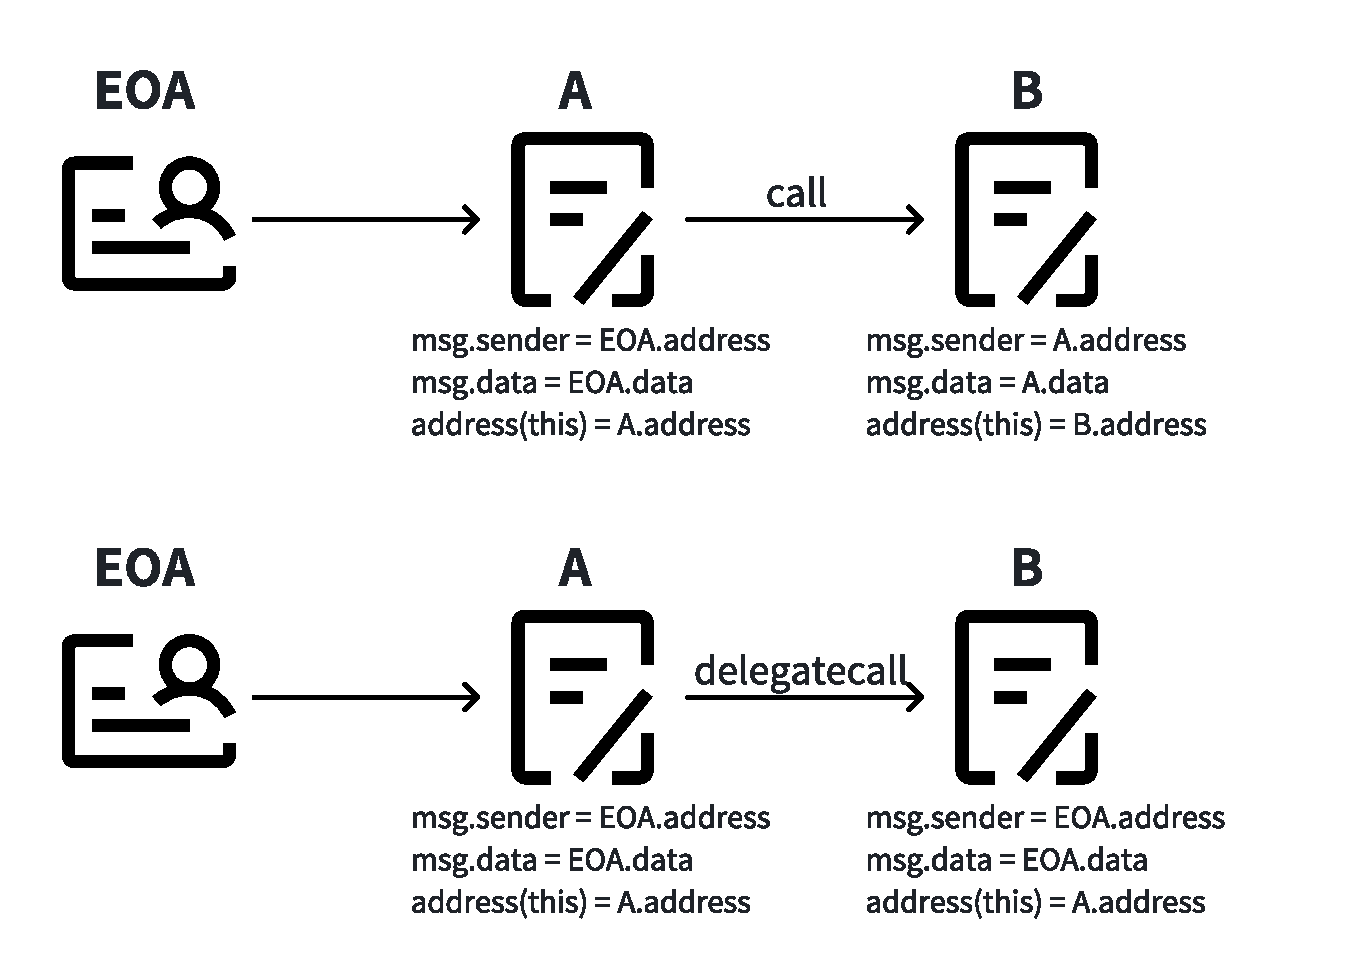
\includegraphics[width=0.45\textwidth]{callVsDelegate.pdf}
    \caption{Comparison of Call and Delegatecall Execution Context}
    \label{fig:call-delegate}
\end{figure}

As shown in Figure \ref{fig:call-delegate}, call() and delegatecall() handle contract addresses and data differently. In call(), the msg.sender becomes the calling contract's address, and the target contract receives this address. However, in delegatecall(), the original caller's address (EOA) is preserved and passed to the target contract. This means that when using delegatecall(), the target contract sees the transaction as if it came directly from the original sender, not from the intermediate contract.

These three call types also differ in their handling of msg.sender:
\begin{itemize}
    \item call(): Changes msg.sender to the calling contract's address
    \item delegatecall(): Keeps the original transaction sender's address
    \item staticcall(): Works like call() but only allows reading data
\end{itemize}

Each method has its specific use case as shown in the table: call() is suitable for general-purpose interactions, delegatecall() is specifically designed for upgrade patterns, and staticcall() is optimized for view functions where state modifications are not needed.

\textbf{Notice}: When implementing upgradeable smart contracts through proxy patterns, delegatecall() is the recommended method as it uniquely maintains the caller's storage context while executing the target contract's logic. This preservation of context is crucial for contract upgradeability, as it allows the proxy contract to maintain its state while delegating the execution of logic to the implementation contract. The method's ability to preserve the original msg.sender ensures proper access control mechanisms remain intact throughout the upgrade process. However, developers must exercise extreme caution when implementing upgradeable contracts using delegatecall(): the storage layout must remain consistent across all contract versions to prevent state corruption, implementation contracts must undergo thorough security audits, and robust access controls must be established for the upgrade functionality to prevent unauthorized modifications.

\vspace{1em}
\subsection{Memory Array vs Storage Array}

\subsubsection{Background and Implementation}
In Solidity, there are various data types including integers (uint/int), addresses (address), booleans (bool), and more. When dealing with multiple values of the same type, arrays provide an efficient way to store and manage these values instead of declaring multiple individual variables. There are two types of arrays: memory arrays and storage arrays, each with distinct characteristics in terms of persistence and mutability.

\begin{lstlisting}[style=solidity]
contract ArrayComparison {
    // Storage array examples with different types
    uint256[] public numbers;      // Array of integers
    address[] public addresses;    // Array of addresses
    bool[] public flags;          // Array of booleans
    
    // Memory array operations
    function memoryArrayOps() public pure returns (uint256[] memory) {
        uint256[] memory memArray = new uint256[](3);
        memArray[0] = 1;
        memArray[1] = 2;
        memArray[2] = 3;
        return memArray;
    }
    
    // Dynamic storage array operations
    function storageArrayOps() public {
        numbers.push(1);    // Dynamic sizing
        numbers.push(2);
        numbers.pop();      // Can remove elements
    }
}
\end{lstlisting}

\subsubsection{Implementation Mechanisms}
Storage arrays are implemented using Ethereum's persistent storage, where elements are stored in non-contiguous slots calculated using the array's base position and element index \cite{solidityStorage}. This allows for dynamic resizing but incurs higher gas costs. In contrast, memory arrays are allocated in a contiguous block of memory during function execution, with a fixed size specified at creation time. The memory layout starts with a 32-byte length field, followed by the array elements, each occupying 32 bytes.

{\small
\begin{verbatim}
Storage Layout:          Memory Layout:
slot p: Length          0x00-0x20: Array length
keccak256(p): Item 0    0x20-0x40: First element
keccak256(p)+1: Item 1  0x40-0x60: Second element
\end{verbatim}
}

\subsubsection{Key Differences}
The fundamental distinction between memory and storage arrays lies in their persistence and mutability. Storage arrays persist between function calls and can be dynamically resized using push() and pop() operations, making them suitable for contract state management. Memory arrays, while more gas-efficient for read and write operations, are temporary and fixed in size, making them ideal for function-scoped computations and return values.

\vspace{1em}
\subsection{Receive vs. Fallback}

\subsubsection{Background and Implementation}
In Solidity, contracts can receive ETH through two special functions: receive() and fallback(). While receive() is specifically designed for plain ETH transfers with no additional data, fallback() serves as a more general-purpose function that handles both function calls with data and ETH transfers when receive() is not present. This dual-purpose nature of fallback() means it can effectively replace receive() in many cases, though at the cost of reduced code clarity and slightly higher gas consumption.

\begin{lstlisting}[style=solidity]
contract PaymentHandler {
    event Received(address sender, uint amount);
    
    // Specific handler for plain ETH transfers
    receive() external payable {
        emit Received(msg.sender, msg.value);
    }
    
    // General-purpose handler for all cases
    fallback() external payable {
        // Can handle both ETH transfers and function calls
        // Has access to msg.data if needed
    }
}
\end{lstlisting}

\subsubsection{Comparative Analysis}
The function selection mechanism in Solidity prioritizes receive() for plain ETH transfers when both functions are present. When a contract receives a transaction with no calldata, the EVM first attempts to execute receive(). Only if receive() is not defined will it fall back to the fallback() function. For calls with data, fallback() is always used unless a matching function signature is found. This hierarchy reflects the design philosophy of having specialized functions for common cases (receive() for plain transfers) while maintaining flexibility through a general-purpose fallback mechanism.

In the Solidity smart contract, receive() and fallback() functions have significant differences in functional scope and application scenarios. receive() function adopts a stricter but purposeful design concept, which is exclusively used to process pure ETH transfer transactions and has no access to transaction data. This specialisation limits the scope of its functionality, but provides a clearer expression of the code's intent when dealing with simple transfer scenarios. In contrast, the fallback() function offers more comprehensive flexibility, not only in terms of being able to handle all types of call requests, but also in terms of accessing msg.data, making it ideal for implementing generic processing logic and custom function routing. However, this flexibility comes at the cost of potentially reducing the clarity of the code's intent, as well as a slightly higher gas cost due to the need to handle call data.

In practice, the choice between implementing both functions or relying only on the fallback() function will largely depend on the contract's specific trade-off between clarity and flexibility needs. The explicit intent of the receive() function may be more valuable for contracts that are primarily concerned with simple ETH receiving functionality, while the flexibility of the fallback() function may be more important for contracts that need to handle complex inbound calls. It is worth noting that in modern smart contract development practice, many contracts choose to implement both functions to ensure functional integrity while keeping concerns separate. This approach not only meets the needs of different scenarios, but also provides better code organisation.
\vspace{3em}  % 添加3个字符高度的垂直空间

\section{Security Analysis}

\subsection{Overflow Vulnerabilities}
In Solidity, arithmetic operations and array bounds can lead to critical security vulnerabilities through overflow or underflow conditions \cite{overflowVuln}. Understanding these vulnerabilities and their prevention mechanisms is essential for secure smart contract development.

\subsubsection{Arithmetic Overflow}
Before Solidity 0.8.0, arithmetic operations could silently overflow, leading to unexpected results. For example:

\begin{itemize}
    \item \textbf{uint8 Overflow}: Maximum value is 0xff (binary: 11111111):
    \[ \text{0xff} + \text{0x01} = \text{1}\text{00000000} \rightarrow \text{00000000} \]
    When adding 1 to 0xff, the result requires 9 bits (100000000), but since uint8 can only store 8 bits, the leading 1 is truncated, resulting in 0x00.
    
    \item \textbf{uint8 Underflow}: Minimum value is 0x00:
    \[ \text{0x00} - \text{0x01} = \text{11111111} = \text{0xff} \]
    When subtracting 1 from 0x00, it borrows from a higher bit, wrapping around to the maximum 8-bit value.
\end{itemize}

To prevent these vulnerabilities, OpenZeppelin's SafeMath library implements checks before each arithmetic operation:

\begin{lstlisting}[style=solidity]
library SafeMath {
    function add(uint256 a, uint256 b) internal pure returns (uint256) {
        uint256 c = a + b;
        require(c >= a, "SafeMath: addition overflow");
        return c;
    }

    function sub(uint256 a, uint256 b) internal pure returns (uint256) {
        require(b <= a, "SafeMath: subtraction overflow");
        return a - b;
    }

    function mul(uint256 a, uint256 b) internal pure returns (uint256) {
        if (a == 0) return 0;
        uint256 c = a * b;
        require(c / a == b, "SafeMath: multiplication overflow");
        return c;
    }
}
\end{lstlisting}

To prevent these vulnerabilities, OpenZeppelin's SafeMath library implements checks before each arithmetic operation. Since Solidity 0.8.0, these checks have been built into the compiler, automatically reverting transactions when overflow occurs. This built-in protection eliminates the need for SafeMath in most cases. However, as discussed in our earlier comparison of SafeMath vs. Native Checks vs. Unchecked, there are scenarios where bypassing these checks through unchecked blocks can optimize gas consumption, particularly in mathematically bounded operations like loop counters.

\subsubsection{Array Bounds}
Memory arrays in Solidity have fixed sizes and require careful bounds checking \cite{solidityStorage}. Attempting to access elements beyond the array's length will cause the transaction to revert. While the EVM automatically enforces these bounds checks, developers should still implement proper validation to prevent unnecessary transaction failures and gas waste.

For dynamic storage arrays, the main security concerns lie in proper length management and access control. While .push() operations are inherently safe, developers need to be cautious about unbounded array growth which could lead to excessive gas costs. Additionally, when deleting elements, using delete directly on array elements can leave gaps in storage, making the swap-and-pop pattern a more efficient and secure approach.

Static arrays, while providing compile-time size guarantees and potentially better gas efficiency, still require careful index validation to prevent out-of-bounds access attempts. Their fixed size nature provides some inherent safety but can be limiting in scenarios requiring dynamic sizing. When copying between static arrays, developers should ensure size compatibility to prevent data truncation.

In both cases, implementing proper bounds checking and size validation is crucial for maintaining contract security, though the specific approaches may differ based on the array type chosen.

\vspace{1em}
\subsection{Replay Attacks}
In the field of smart contract security, replay attacks are a way of achieving unintended effects by maliciously repeating valid transactions, and Solidity mitigates the risk of such attacks by providing multiple layers of protection through its design features and built-in mechanisms.

The 2300 gas limit enforced by the transfer() and send() functions, while originally designed to prevent reentry attacks, also constitutes an effective barrier against replay attacks. This gas limit ensures that the receiving contract can only perform minimal logical operations, typically limited to recording the receipt of funds, and cannot initiate external calls or complex state changes that could be exploited by a replay attack.

Similarly, the gas limitations of the receive() and fallback() functions provide inherent protection mechanisms. receive() functions are specifically designed to handle pure ETH transfers, and their limited execution environment inherently reduces the risk of replay attacks. The fallback() function, on the other hand, while offering greater flexibility, can be effectively prevented from becoming an attack vector through proper gas management and implementation models.

However, the more flexible call() method, which does not enforce gas restrictions, requires developers to take additional security measures in its implementation. When using call(), it is recommended to implement the following protection mechanisms:
\begin{itemize}
\item Maintain counters for each operation using a nonce tracking mechanism

\item Implement reasonable transaction time window validation

\item Establish fine-grained function access control to limit the calling privileges of specific functions
\end{itemize}

These security considerations demonstrate how Solidity's built-in features, when used appropriately, can effectively protect against replay attacks while maintaining contract functionality. By using these mechanisms together, developers can build more secure and robust smart contract systems.

\vspace{1em}
\subsection{Storage Layout Conflicts}
When using delegatecall, one of the most critical security vulnerabilities arises from storage layout conflicts \cite{storageLayout}. Since delegatecall executes the target contract's code in the context of the calling contract's storage, mismatched storage layouts can lead to unintended state modifications \cite{proxyPatterns}. Consider this example:

\begin{lstlisting}[style=solidity]
// Original Contract
contract Logic {
    address public owner;    // slot 0
    uint256 public value;    // slot 1
}

// Updated Contract (Incorrect Layout)
contract LogicV2 {
    uint256 public value;    // slot 0 - Will overwrite owner!
    address public owner;    // slot 1
}
\end{lstlisting}

In this example, if a proxy contract using delegatecall upgrades from Logic to LogicV2, any operation modifying the value variable in LogicV2 will accidentally corrupt the owner variable in the proxy's storage due to the misaligned storage slots. This type of vulnerability can lead to severe security issues, including loss of contract ownership or corruption of critical state variables.

To prevent such vulnerabilities:
\begin{itemize}
    \item Always maintain consistent storage layouts across contract versions
    \item Implement thorough testing of storage layouts before deployment
\end{itemize}

\vspace{3em}
\section{Gas Analysis}
\subsection{\textbf{environment}}
We use multiple tools and platforms for testing:
\begin{itemize}
    \item Tenderly platform: for contract deployment and trade simulation (\url{https://dashboard.tenderly.co/explorer})
    \item Remix IDE: for contract compilation and initial testing (\url{https://remix.ethereum.org})
    \item MetaMask: for testing network deployment
    \item Python matplotlib: for data visualization
\end{itemize}

Due to limited testnet tokens, we utilized Tenderly for simulated transactions, which provides detailed transaction information. For each simulated transaction, we performed 5 iterations to obtain average data and minimize variance.

\vspace{1em}
\subsection{\textbf{Analysis}}
Firstly,We tested the gas cost data for assert, require, and revert methods across versions 0.7.0 and 0.8.0. Figure \ref{fig:version-comparison} shows our findings.

\begin{figure}[htbp]
    \centering
    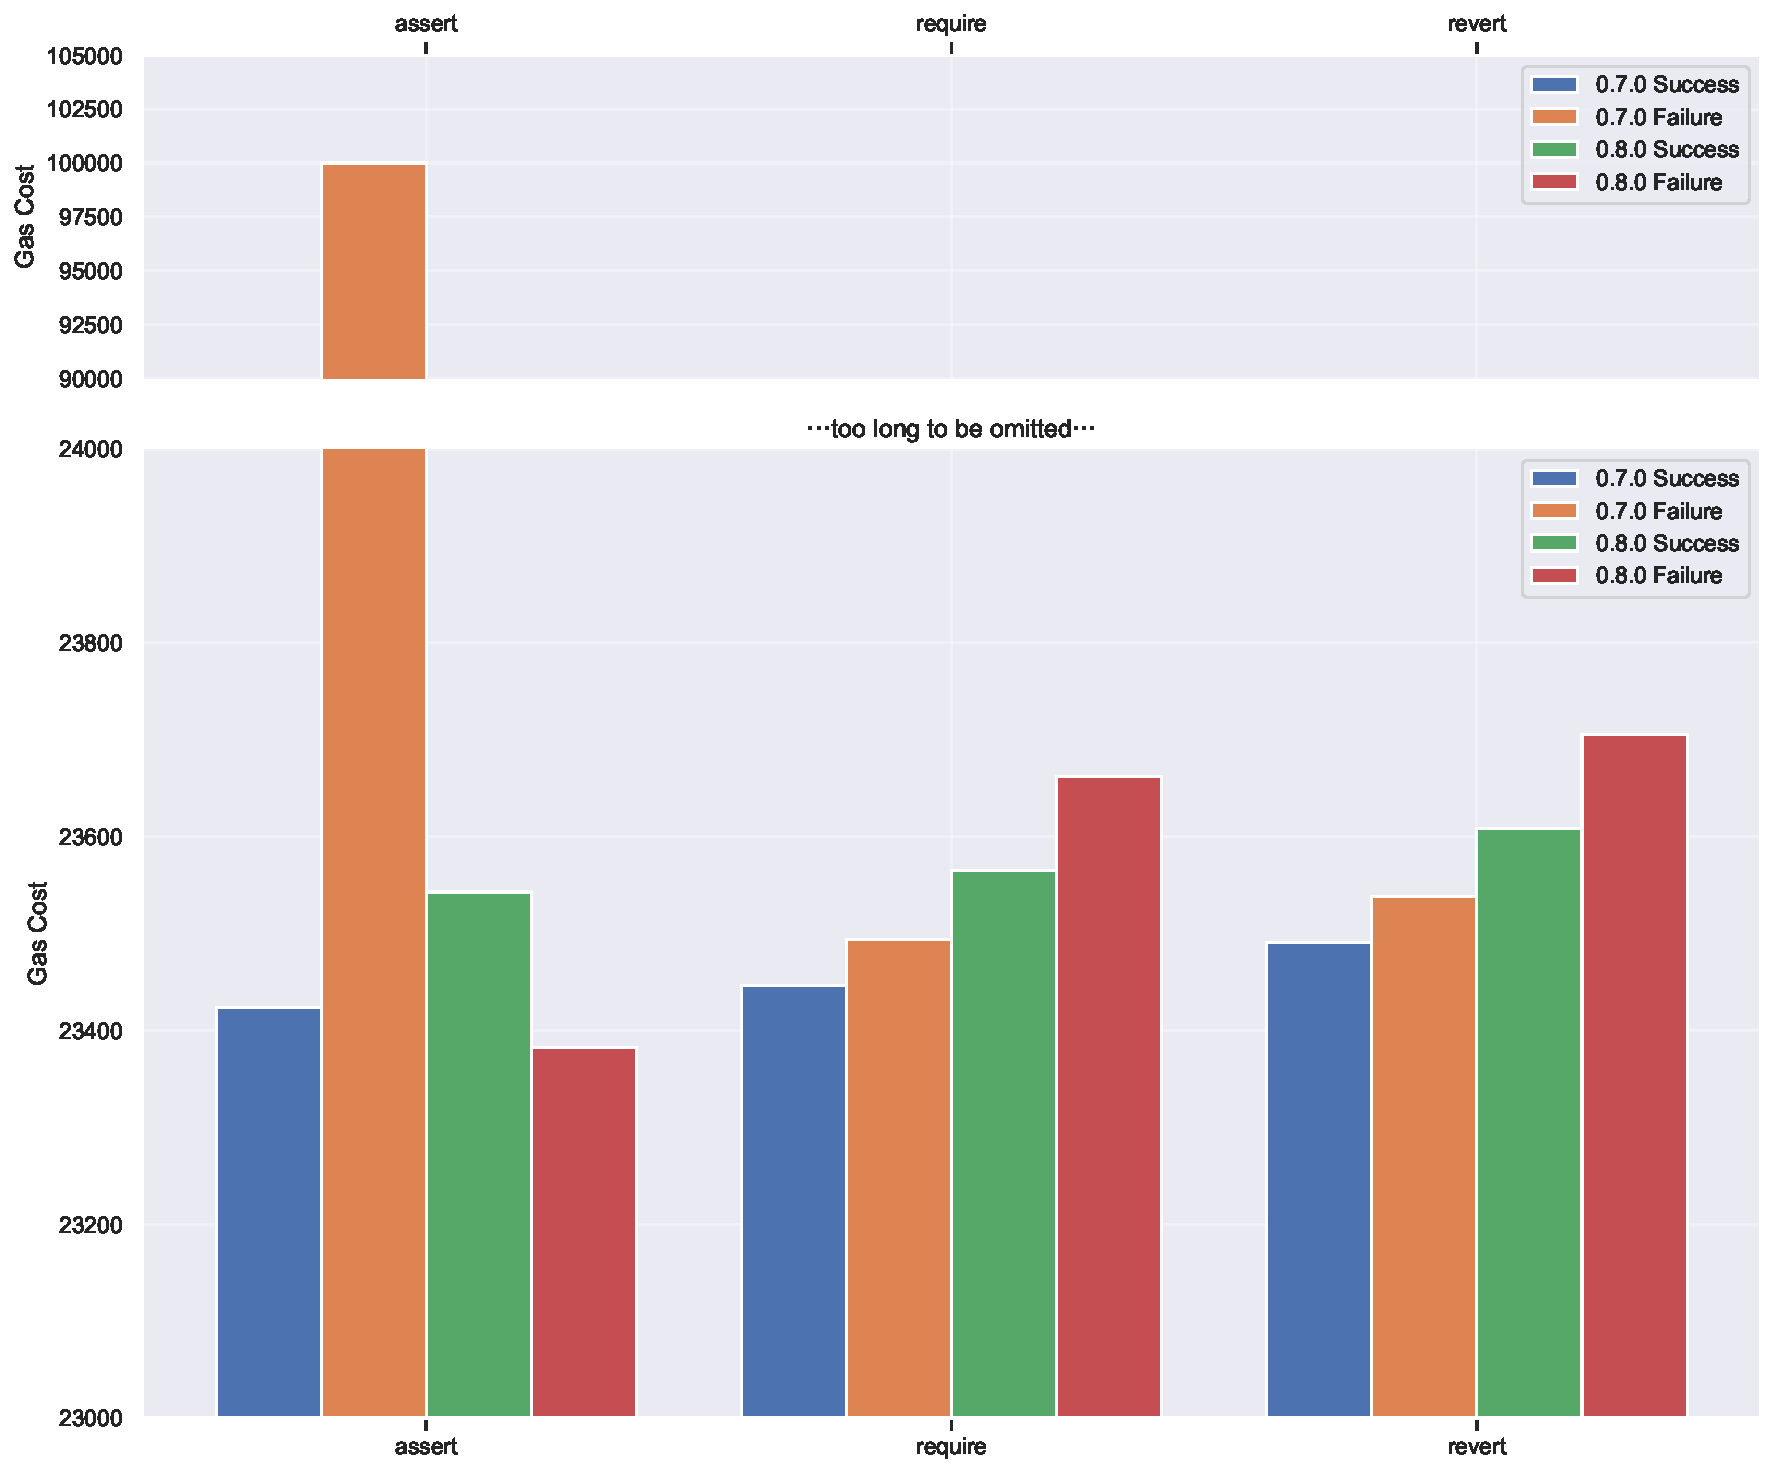
\includegraphics[width=0.45\textwidth]{version_comparison.pdf}
    \caption{Gas Cost Comparison Across Solidity Versions}
    \label{fig:version-comparison}
\end{figure}

We can see that failures tend to consume more gas than successes, this is due to the fact that the rollback operation after a failure consumes a certain amount of gas fee. Due to the extra security checks added to these functions in version 0.8.0, the compiler generates more opcodes to handle boundary cases, so higher versions consume more gas for the same state. An exception, we found that failing an assert transaction consumes all the gas in versions below 0.8.0, so developers should be more willing to spend a little bit more gas to get a more secure review mechanism to avoid excessive losses.

\vspace{1em}
Next, We also compared gas costs between using modifiers and direct function validation, as shown in Table \ref{tab:modifier-comparison}.

\begin{table}[htbp]
\renewcommand{\arraystretch}{1.2}
\centering
\caption{Gas Cost Comparison: Modifiers vs Direct Validation}
\begin{tabular}{|l|c|c|}
\hline
\textbf{Validation Method} & \textbf{Success (gas)} & \textbf{Failure (gas)} \\
\hline
Direct Validation & 23,542 & 23,639 \\
\hline
Modifier & 23,586 & 23,683 \\
\hline
\end{tabular}
\label{tab:modifier-comparison}
\end{table}

The result shows that although modifiers consume a little bit more, this is due to the fact that modifiers are essentially code inlining, and the compiler will insert the modifier code directly into the function. The final compiled bytecode is very similar, except for the extra jump instruction, it usually only consumes about 20-50 gas more, but in view of the advantages of modifiers analyzed above, this article suggests that they can all be expressed as modifiers, unless there are too many a priori conditions, and nesting modifiers in multiple layers may lead to errors, so we can use in-function conditions.

\vspace{1em}
Since the problem of overflow above and below a function is very serious and can lead to contractually fatal errors, we have analysed the cost of gas consumed by safely adding and subtracting maths, and the results are shown in Figure \ref{fig:arithmetic-comparison}.

\begin{figure}[htbp]
    \centering
    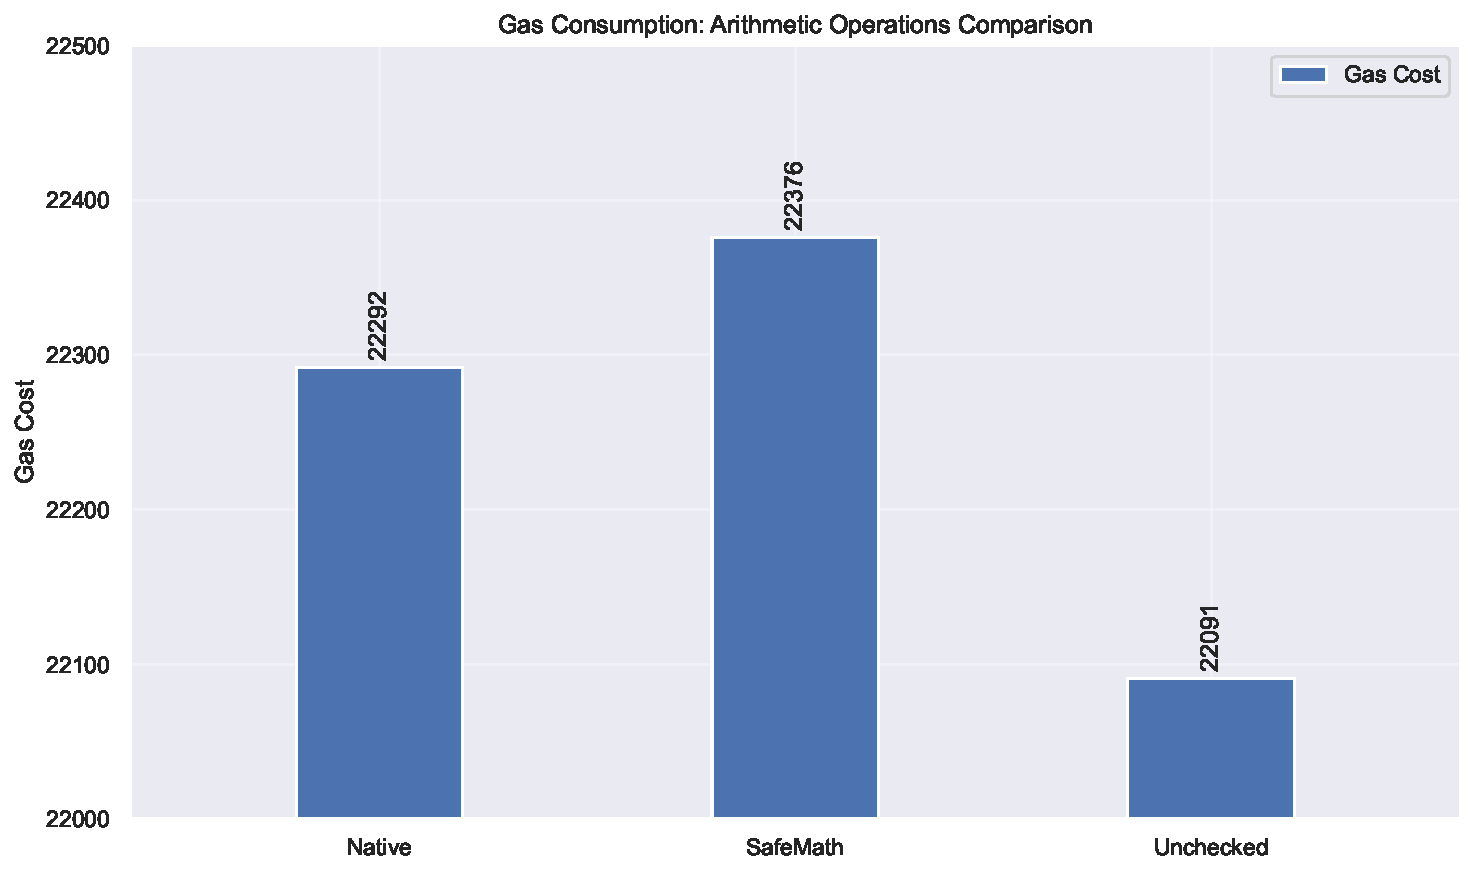
\includegraphics[width=0.45\textwidth]{arithmetic_comparison.pdf}
    \caption{Gas Cost Comparison: Arithmetic Safety Mechanisms}
    \label{fig:arithmetic-comparison}
\end{figure}

Because we are using version 0.8.0 or above, the compiler has been optimized, although it is not as big as the above comparative analysis of the gas difference, but the size of the gas cost can still reflect the performance of different methods, as we said above, unchecked consumes the smallest cost, safemath consumes the largest cost. 

\vspace{1em}
In Ether smart contracts, ETH is closely related to the method of sending ETH, so we have also analyzed transfer methods: Figure \ref{fig:transfer-comparison}.

\begin{figure}[htbp]
    \centering
    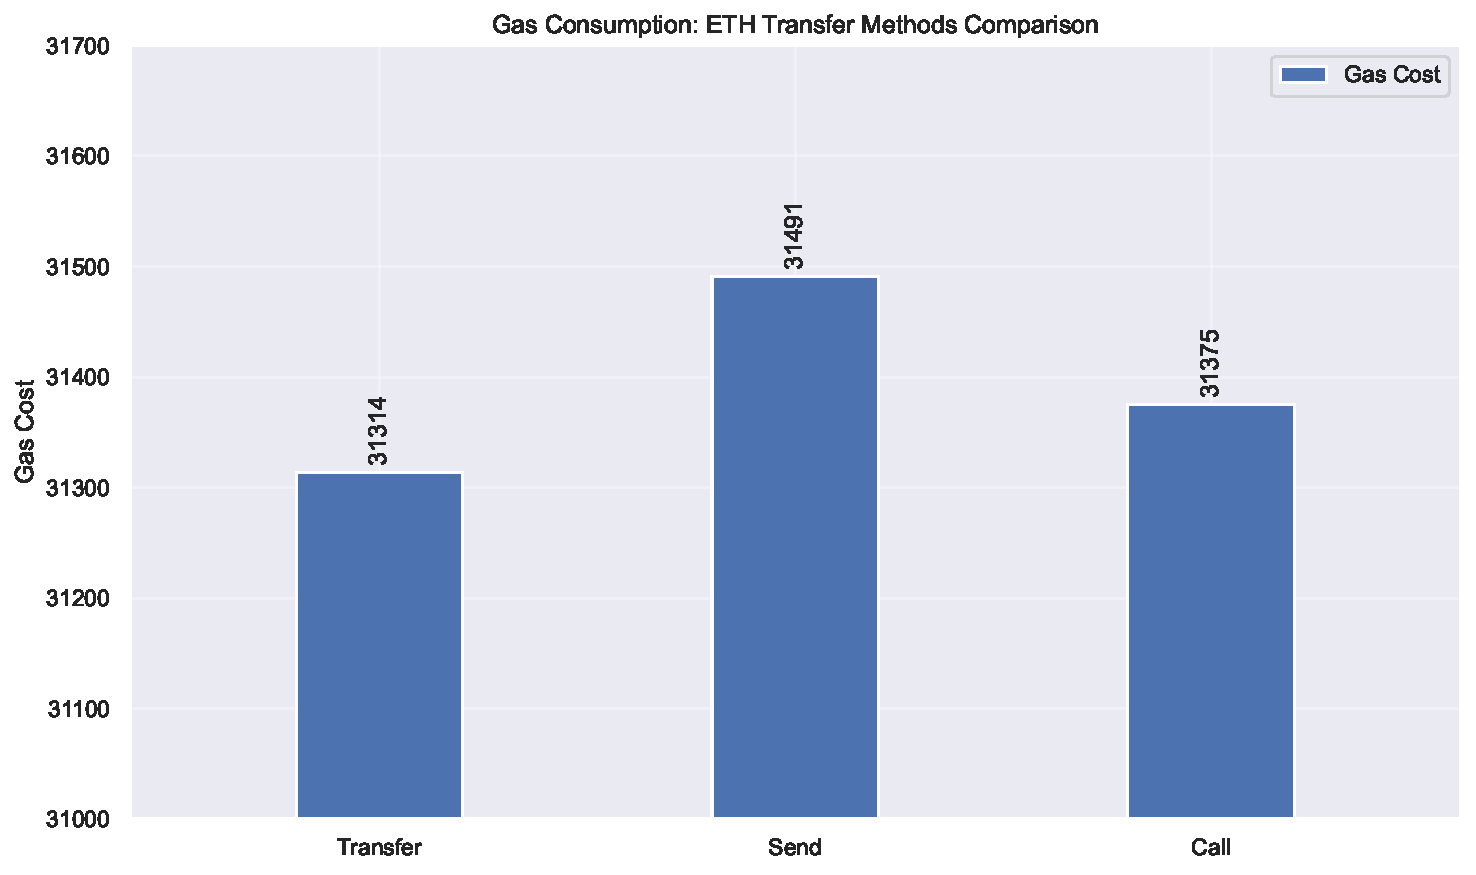
\includegraphics[width=0.45\textwidth]{transfer_comparison.pdf}
    \caption{Gas Cost Comparison: ETH Transfer Methods}
    \label{fig:transfer-comparison}
\end{figure}

The reason why transfer is lowest is that we use a fixed sequence of opcodes, which the compiler can optimize, and do not need to handle return values, and failure is rolled back directly without additional error handling logic, whereas send needs to handle boolean return values and includes an additional return value checking mechanism.

\vspace{1em}
\textbf{Notice:} Of course, first of all, to ensure that the contract security premise, the developer needs to further consider the gas optimisation problem, and different versions have different methods of application, developers need to always pay attention to the

\vspace{3em}
\section{Conclusion}
This paper provides an in-depth analysis of the different functional implementation alternatives commonly encountered by Solidity beginners. By examining seven pairs of key alternatives, we observe that the built-in compiler checks for smart contracts have become increasingly comprehensive and sophisticated with major upgrades to the Solidity release. However, developers should not be overly reliant on these automated checking mechanisms, but should instead keep an eye on the functionality changes in each major version update. This in-depth understanding of version changes enables developers to make appropriate adjustments in different versions of smart contracts to ensure contract security.

In addition to security considerations, developers need to maintain a balance between code reusability and efficiency, focusing on gas optimization. By following the design principles of high cohesion and low coupling, developers can establish good programming practices and lay a solid foundation for advanced smart contract development. This systematic approach not only improves the maintainability of contracts, but also provides the necessary technical support for building complex decentralized applications.

\vspace{3em}
% Move bibliography to the end
\begin{thebibliography}{2}
\bibitem{wikiSolidity}
    Wikipedia Contributors,
    ``Solidity,''
    Wikipedia, The Free Encyclopedia,
    2024.
    [Online].
    Available: \url{https://en.wikipedia.org/wiki/Solidity}
    
\bibitem{solidity080}
    Solidity Team, 
    ``Solidity 0.8.0 Breaking Changes,'' 
    Solidity Documentation, 
    2020. 
    [Online]. 
    Available: \url{https://docs.soliditylang.org/en/v0.8.0/080-breaking-changes.html}

\bibitem{solidityModifiers}
    Solidity Team,
    ``Solidity Modifiers,''
    Solidity Documentation,
    2020.
    [Online].
    Available: \url{https://docs.soliditylang.org/en/v0.8.0/070-inheritance.html#modifiers}

\bibitem{openzeppelin}
    OpenZeppelin Team,
    ``SafeMath Library,''
    OpenZeppelin Documentation,
    2020.
    [Online].
    Available: \url{https://github.com/OpenZeppelin/openzeppelin-contracts/blob/master/contracts/utils/math/SafeMath.sol}

\bibitem{solidityArithmetic}
    Solidity Team,
    ``Arithmetic in Solidity,''
    Solidity Documentation,
    2023.
    [Online].
    Available: \url{https://docs.soliditylang.org/en/v0.8.0/control-structures.html#checked-or-unchecked-arithmetic}

\bibitem{transferComparison}
    Solidity Team,
    ``Address Members,''
    Solidity Documentation,
    2023.
    [Online].
    Available: \url{https://docs.soliditylang.org/en/v0.8.17/types.html?highlight=send#members-of-addresses}

\bibitem{transferMedium}
    Z. Mohammed,
    ``Solidity — transfer vs send vs call function,''
    Coinmonks,
    Dec. 2021.
    [Online].
    Available: \url{https://medium.com/coinmonks/solidity-transfer-vs-send-vs-call-function-64c92cfc878a}

\bibitem{callTypes}
    Solidity Team,
    ``Contract ABI Specification,''
    Solidity Documentation,
    2023.
    [Online].
    Available: \url{https://docs.soliditylang.org/en/v0.8.17/abi-spec.html#function-selector-and-argument-encoding}

\bibitem{solidityStorage}
    Solidity Team,
    ``Solidity Storage and Memory,''
    Solidity Documentation,
    2023.
    [Online].
    Available: \url{https://docs.soliditylang.org/en/v0.8.17/internals/layout_in_memory.html}

\bibitem{overflowVuln}
    N. Atzei, M. Bartoletti, and T. Cimoli,
    ``A Survey of Attacks on Ethereum Smart Contracts,''
    Principles of Security and Trust,
    2017.
    [Online].
    Available: \url{https://doi.org/10.1007/978-3-662-54455-6_8}

\bibitem{replayAttacks}
    G. Chen et al.,
    ``Understanding Ethereum via Graph Analysis,''
    IEEE INFOCOM,
    2018.
    [Online].
    Available: \url{https://doi.org/10.1109/INFOCOM.2018.8486401}

\bibitem{storageLayout}
    F. Zhang et al.,
    ``Smart Contract Security: A Software Lifecycle Perspective,''
    IEEE Access,
    vol. 7,
    pp. 150184-150202,
    2019.
    [Online].
    Available: \url{https://doi.org/10.1109/ACCESS.2019.2946988}

\bibitem{proxyPatterns}
    OpenZeppelin Team,
    ``Proxy Upgrade Pattern,''
    OpenZeppelin Documentation,
    2021.
    [Online].
    Available: \url{https://docs.openzeppelin.com/upgrades-plugins/1.x/proxies}

\bibitem{githubRepo}
    SHAO Yuning,
    ``In-Depth Analysis in Solidity Smart Contracts,''
    GitHub Repository,
    2024.
    [Online].
    Available: \url{https://github.com/RootCoinT/In-Depth-Analysis-in-Solidity-Smart-Contracts}
    
\end{thebibliography}

\end{document}